\section{Semaphore}
\begin{figure} [ht]
	\centerline{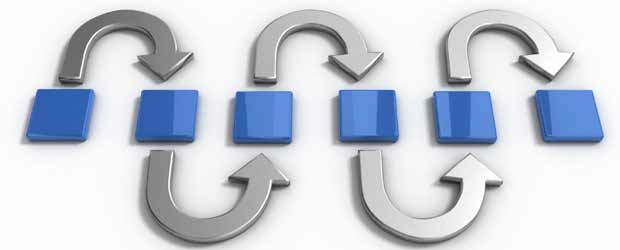
\includegraphics[width=1\textwidth]{figures/proses.jpg}}
	\caption{Gambar Hirarki Semaphore}
	\label{SemaphoreHirarki}
\end{figure}

Semaphore merupakan struktur data yang digunakan untuk mensinkronisasikan proses yang ada pada sebuah komputer, yang memiliki proses yang dijalankan lebih dari satu dan melakukan proses tersebut secara bersamaan dan teratur urutan kerjanya \ref{SemaphoreHirarki}. Dalam sistem proses data, banyak dari simpul berbagi sumber daya. 
Semaphore sendiri adalah sebuah variabel dengan tipe data bilangan bulat atau integer, Dalam kehidupan nyata, semaphore adalah sistem sinyal yang digunakan untuk berkomunikasi secara visual. 
\cite{zuberi1997efficient}Dalam pemrograman berbasis obyek, memperbaharui dari penegasan variabel dari obyek dapat dilindungi melalui semaphore untuk memastikan pengecualian. Operasi semaphore dipanggil setiap obyek diakses, dan ini menampilkan pengeluaran yang signifikan.
\break Dalam pemrograman semaphore dapat diakses menggunakan operasi ini :
\begingroup\makeatletter\def\@currenvir{verbatim}
\verbatim
P(Semaphore s)
{
  wait until s > 0, then s := s-1;
  /* must be atomic once s > 0 is detected */
}

V(Semaphore s)
{
  s := s+1;   /* must be atomic */
}

Init(Semaphore s, Integer v)
{
  s := v;
}
\end{verbatim}


\subsection{Jenis Semaphore}
Semaphore memiliki 2 jenis, diantaranya:
\begin{enumerate}
	\item Binary semaphore \\ Semaphore ini hanya memiliki nilai 1 atau 0. atau sering disebut semaphore primitif
	\item Counting semaphore.\\ Semaphore ini memiliki nilai 0, 1, serta integer lainnya.
\end{enumerate}

Rata-rata sistem operasi yang menggunakan binary semaphore saja sebagai primitif, tetapi  yang menggunakan counting semaphore dibuat dengan memakai primitif ini.
Harus diketahui di sini bahwa, ada beberapa jenis dari counting semaphore. Salah satu jenis counting semaphore ini adalah yang tidak mencapai nilai negatif Jenis yang lain adalah semaphore yang dapat mencapai nilai negatif.


Keuntungan dalam menggunakan semaphore :

\begin{itemize}
	\item Penanganan masalah dan sinkronisasi lebih teratur sehinggan mudah untuk dicari kebenarannya.
	\item Penggunaan semaphore bersifat portable karena implementasi semaphore ke dalam hard code.
\end{itemize}
	
	Kerugian dalam menggunakan semaphore :
	
	\begin{itemize}
		\item Pemeliharaan yang cukup sulit karena tersebar di seluruh program.
		\item Memungkinkan terjadinya non  mutual exclusion dan deadlock.
		\item Penanganan error yang lebih sulit.
	\end{itemize}
\section{Semaphore memory}
\cite{earnshaw1991semaphore}Penemuan dari semaphore memory dengan pesat mengurangi pertikaian atau bentrok antar bus dengan membolehkan semaphore bit test dan set operations untuk berperforma dalam setiap bus lokal dalam CPU. Semaphore lock bits disimpan dalam SRAM kecepatan tinggi dalam setiap CPU atau Proessor, dan koherensi dari 
lock bits telah diatur dari bus monitoring logic pada setiap CPU. Sebuah CPU berharap untuk mengambil alih sebuah semaphore yang melakukan pembacaan lokal dalam semaphore memory itu sendiri, dan berputar sampai lock bit sudah direset pada waktu dimana pembacaan lokal dilakukan untuk mensetting bit.

\section {Kesimpulan}
1. Semaphore adalah sebuah cara kerja sistem yang efektif dan digunakan baik pada sistem uniprosesor dan atau sistem multiprosesor. Semaphore pada dasarnya adalah counter yang penyajian pesannya hampir selalu menggunakan struktur data.
2. Semaphore merupakan variable data bertipe integer yang dapat diakses menggunakan 2 operasi atomik standar, yaitu wait dan signal.
